\section*{Part A: Solved Examples 1 to 3}

%---------------------------------------------------------------
\subsection*{Example 1}
\textbf{Question.} Prove that in two concentric circles, the chord of the larger circle, which touches the smaller circle, is bisected at the point of contact.

\begin{center}
\begin{tikzpicture}[scale=0.9]
\coordinate (O) at (0,0);
\draw (O) circle (2); \draw (O) circle (1.3);
\coordinate (P) at (-50:1.3);
\coordinate (A) at ($(P)+(40:{sqrt(4-1.69)})$);
\coordinate (B) at ($(P)-(40:{sqrt(4-1.69)})$);
\draw (A) -- (B);
\draw[dashed] (O) -- (P);
\dotat{O}{above left}\dotat{P}{below left}\dotat{A}{above right}\dotat{B}{below}
\node at (130:1.65) {\small $C_2$}; \node at (60:2.35) {\small $C_1$};
\end{tikzpicture}%
\figcap{Concentric circles $C_1$ (larger) and $C_2$ (smaller); chord $AB$ of $C_1$ touches $C_2$ at $P$. Dashed line: construction.}
\end{center}

\Needspace{14\baselineskip}
\textbf{Solution.}

\textbf{Given:} Two concentric circles $C_1$ and $C_2$ with centre $O$. $AB$ is a chord of the larger circle $C_1$ and touches the smaller circle $C_2$ at $P$.

\textbf{To prove:} $AP=BP$.

\textbf{Construction:} Join $OP$.

\proofhd{}
\begin{prf}
1 & $AB$ is a tangent to $C_2$ at $P$ and $OP$ is the radius of $C_2$ through $P$, so $OP\perp AB$. & The tangent to a circle is perpendicular to the radius through the point of contact. \\
2 & $AB$ is a chord of $C_1$ and $OP\perp AB$, where $O$ is the centre of $C_1$. & The perpendicular from the centre of a circle to a chord bisects the chord. \\
3 & $AP=BP$. & From step 2.
\end{prf}

\slip{The perpendicular is drawn from the centre $O$ of the \emph{larger} circle, and the radius $OP$ used is the radius of the \emph{smaller} circle (it ends at the point of contact). Do not mix up which circle each fact refers to.}

\ans{$AP=BP$, so the chord $AB$ is bisected at the point of contact $P$. (Proved)}

\textbf{Alternative proof (without the chord property).} In $\tri OPA$ and $\tri OPB$: $\ang OPA=\ang OPB=90\deg$ (step 1), $OA=OB$ (radii of $C_1$), and $OP$ is common. So $\tri OPA\cong\tri OPB$ (RHS), and $AP=BP$ (CPCT).

%---------------------------------------------------------------
\subsection*{Example 2}
\textbf{Question.} Two tangents $TP$ and $TQ$ are drawn to a circle with centre $O$ from an external point $T$. Prove that $\ang PTQ=2\ang OPQ$.

\begin{center}
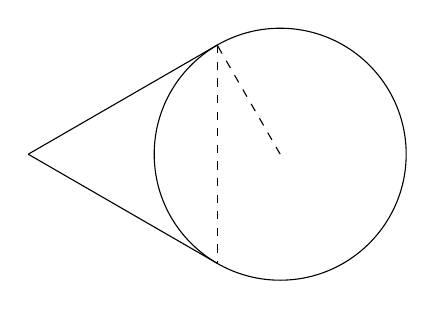
\begin{tikzpicture}[scale=1.0]
\coordinate (O) at (0,0);
\draw (O) circle (1.6);
\coordinate (T) at (-3.2,0);
\coordinate (P) at (120:1.6);
\coordinate (Q) at (240:1.6);
\draw (T) -- (P); \draw (T) -- (Q);
\draw[dashed] (P) -- (Q); \draw[dashed] (O) -- (P);
\dotat{O}{right}\dotat{T}{left}\dotat{P}{above}\dotat{Q}{below}
\end{tikzpicture}%
\figcap{$TP$ and $TQ$ are tangents; $P$ and $Q$ are the points of contact. Dashed lines: construction.}
\end{center}

\textbf{Solution.}

\textbf{Given:} A circle with centre $O$; an external point $T$; tangents $TP$ and $TQ$ with points of contact $P$ and $Q$.

\textbf{To prove:} $\ang PTQ=2\ang OPQ$.

\textbf{Construction:} Join $PQ$ and $OP$.

\proofhd{} Let $\ang PTQ=\theta$.
\begin{prf}
1 & $TP=TQ$. & The lengths of the two tangents from an external point are equal. \\
2 & $\ang TPQ=\ang TQP$. & Angles opposite equal sides of $\tri TPQ$ are equal. \\
3 & $\ang TPQ+\ang TQP+\theta=180\deg$. & Angle-sum property of $\tri TPQ$. \\
4 & $\ang TPQ=\tfrac12(180\deg-\theta)=90\deg-\tfrac12\theta$. & From steps 2 and 3. \\
5 & $\ang OPT=90\deg$. & The tangent is perpendicular to the radius through the point of contact. \\
6 & $\ang OPQ=\ang OPT-\ang TPQ$. & Ray $PQ$ lies inside $\ang OPT$. \\
7 & $\ang OPQ=90\deg-\left(90\deg-\tfrac12\theta\right)=\tfrac12\theta$. & From steps 4, 5 and 6. \\
8 & $\theta=2\ang OPQ$. & From step 7.
\end{prf}

\slip{In step 6 the angle $\ang OPQ$ is the \emph{difference} $\ang OPT-\ang TPQ$, not the sum. Also, $\ang OPT=90\deg$ only because $OP$ is a radius and $TP$ a tangent at the same point $P$.}

\ans{$\ang PTQ=2\ang OPQ$. (Proved)}

%---------------------------------------------------------------
\subsection*{Example 3}
\textbf{Question.} $PQ$ is a chord of length $8$ cm of a circle of radius $5$ cm. The tangents at $P$ and $Q$ intersect at a point $T$. Find the length $TP$.

\begin{center}
\begin{tikzpicture}[scale=0.45]
\coordinate (O) at (0,0);
\draw (O) circle (5);
\coordinate (P) at (3,4); \coordinate (Q) at (3,-4);
\coordinate (T) at ({25/3},0); \coordinate (R) at (3,0);
\draw (T) -- ($(T)!1.1!(P)$);
\draw (T) -- ($(T)!1.1!(Q)$);
\draw (P) -- (Q); \draw (O) -- (P);
\draw[dashed] (T) -- (O);
\draw pic[draw,angle radius=0.3cm] {right angle=O--P--T};
\dotat{O}{below left}\dotat{T}{right}\dotat{P}{above}\dotat{Q}{below}\dotat{R}{below right}
\node[font=\small,above left] at (1.5,2.1) {$5$ cm};
\end{tikzpicture}%
\figcap{Chord $PQ=8$ cm, radius $OP=5$ cm; tangents at $P$ and $Q$ meet at $T$. Dashed line: construction ($OT$ meets $PQ$ at $R$).}
\end{center}

\textbf{Solution.} Join $OT$ and let it meet $PQ$ at $R$.

\textbf{Step 1: $R$ is the mid-point of $PQ$.} $TP=TQ$ (tangents from an external point are equal), so $\tri TPQ$ is isosceles, and $TO$ bisects $\ang PTQ$ (the centre lies on the bisector of the angle between the tangents). The bisector of the vertex angle of an isosceles triangle is perpendicular to the base and bisects it. Hence $OT\perp PQ$ and
\[PR=RQ=\tfrac12\times 8=4\text{ cm}.\]

\textbf{Step 2: find $OR$.} In the right triangle $ORP$ ($\ang ORP=90\deg$), by the Pythagoras theorem $OP^2=OR^2+PR^2$:
\begin{align*}
OR^2&=OP^2-PR^2=5^2-4^2=25-16=9\\
OR&=\sqrt9=3\text{ cm}.
\end{align*}
\slip{The hypotenuse of $\tri ORP$ is $OP$ (opposite the right angle at $R$), so $OP^2$ is the sum, and $OR^2=OP^2-PR^2$ is a difference. Writing $5^2+4^2$ here is wrong.}

\textbf{Step 3: two equal angles} (this answers the book's ``Why?''). The tangent is perpendicular to the radius, so $\ang TPO=90\deg$, i.e.
\[\ang TPR+\ang RPO=90\deg.\]
In $\tri TRP$, $\ang TRP=90\deg$, so by the angle-sum property
\[\ang TPR+\ang PTR=90\deg.\]
Comparing the two, $\ang RPO=\ang PTR$.

\textbf{Step 4: similar triangles.} In $\tri TRP$ and $\tri PRO$: $\ang TRP=\ang PRO=90\deg$ and $\ang PTR=\ang RPO$ (Step 3). So $\tri TRP\sim\tri PRO$ (AA similarity), and corresponding sides are proportional:
\[\frac{TP}{PO}=\frac{RP}{RO}\ \Rightarrow\ \frac{TP}{5}=\frac{4}{3}\ \Rightarrow\ TP=\frac{20}{3}\text{ cm}.\]

\textbf{Verification.} In the right triangle $TRP$ (right angle at $R$), by the Pythagoras theorem $TR^2=TP^2-PR^2$:
\[TR^2=\left(\frac{20}{3}\right)^2-4^2=\frac{400}{9}-\frac{144}{9}=\frac{256}{9},\qquad TR=\frac{16}{3}\text{ cm}.\]
So $OT=TR+RO=\dfrac{16}{3}+3=\dfrac{25}{3}$ cm. In $\tri OPT$, by the Pythagoras theorem $OT^2=TP^2+OP^2$ should hold:
\[TP^2+OP^2=\left(\frac{20}{3}\right)^2+5^2=\frac{400}{9}+\frac{225}{9}=\frac{625}{9},\qquad OT^2=\left(\frac{25}{3}\right)^2=\frac{625}{9}.\]
Both sides are equal, so the answer is correct.

\ans{$TP=\dfrac{20}{3}$ cm $\left(=6\tfrac23\text{ cm}\right)$.}

\textbf{Alternative solution (Pythagoras theorem).} Let $TP=x$ and $TR=y$, so $OT=TR+RO=y+3$.

In the right triangle $PRT$ (right angle at $R$), $TP^2=TR^2+PR^2$ with $PR=4$:
\[x^2=y^2+4^2=y^2+16.\]
In the right triangle $OPT$ (right angle at $P$), $OT^2=TP^2+OP^2$ with $OP=5$:
\[(y+3)^2=x^2+5^2=x^2+25.\]
Expand the left side by the identity $(a+b)^2=a^2+2ab+b^2$, giving $(y+3)^2=y^2+2\cdot y\cdot3+3^2=y^2+6y+9$, and put $x^2=y^2+16$ on the right:
\begin{align*}
y^2+6y+9&=(y^2+16)+25\\
y^2+6y+9&=y^2+41\\
6y&=41-9=32\\
y&=\frac{32}{6}=\frac{16}{3}.
\end{align*}
Then, putting $y=\dfrac{16}{3}$ and writing $16=\dfrac{144}{9}$:
\[x^2=\left(\frac{16}{3}\right)^2+16=\frac{256}{9}+\frac{144}{9}=\frac{400}{9},\qquad x=\sqrt{\frac{400}{9}}=\frac{20}{3}\text{ cm}.\]
